\documentclass[12pt]{article}
\usepackage{amssymb}
\usepackage{amsmath}
\usepackage{bm} % bold maths
\usepackage[normalem]{ulem} % cross stuff out
\usepackage{tikz} % for diagrams
\usepackage[font={it},justification=centering]{caption}% italic figure captions
%\usepackage{natbib}
%\usepackage{har2nat}
%\usepackage[style=authoryear,backend=biber]{biblatex}
%\usepackage{harvard}


\newcommand{\HRule}{\rule{\linewidth}{0.5mm}} % rule horizontal line
\usepackage[]{algorithmic}
\usepackage{algorithm}
%\usepackage{alg-pseudocode}
%\usepackage[numbered]{algo}


\DeclareMathOperator*{\argmax}{arg\,max\,}


\usepackage{fancyhdr}%to have a header and footer
%\pagestyle{fancy}

%\usepackage{longtable} % to split tables over the page

\usepackage{setspace}%this stops lists having so much gap in them
\usepackage{enumitem}
\setlist{nolistsep}


% for xfig
\usepackage{graphicx}
%\usepackage[usenames,dvipsnames]{color}
%\usepackage[pdftex]{graphicx}
%\DeclareGraphicsExtensions{.pdf, .jpg}
%\usepackage{epsfig}
% end for xfig

\usepackage[mathscr]{eucal}%Euler script, use \mathscr


% external references
%\usepackage{xr}
%\externaldocument[TS-]{tgt-splash-paper}

\setlength{\topmargin}{-1.5cm} 
\setlength{\textheight}{22cm}
\setlength{\oddsidemargin}{-0.2cm}
\setlength{\evensidemargin}{-1.2cm} 
\setlength{\textwidth}{16cm}
\setlength{\parindent}{0pt}
\setlength{\parskip}{.35cm}


\newtheorem{theorem}{Theorem}[section]
\newtheorem{lemma}[theorem]{Lemma}
\newtheorem{corollary}[theorem]{Corollary}
\newtheorem{defn}[theorem]{Definition}
\newtheorem{definition}[theorem]{Definition}
\newtheorem{example}[theorem]{Example}
\newtheorem{remark}[theorem]{Remark}
\newtheorem{construction}{Construction}
\newtheorem{conjecture}[theorem]{Conjecture}
\newtheorem{result}[theorem]{Result}
\newenvironment{proof}{\noindent{\bf Proof}\hspace{0.5em}}
    { \null  \hfill $\square$ \par}


\newcommand{\B}{\mathcal B}
\newcommand{\X}{\mathcal X}
\newcommand{\Y}{\mathcal Y}
\newcommand{\R}{\mathcal R}
\newcommand\C{{\cal C}}
\newcommand\E{{\cal E}}
\newcommand\I{{\cal I}}
\newcommand\D{{\cal D}}
\newcommand\F{{\cal F}}
\newcommand\N{{\cal N}}
\newcommand\J{{\cal J}}
\renewcommand\L{{\mathscr L}}
\renewcommand{\S}{\mathcal S}
\renewcommand{\P}{\mathcal P}
\newcommand{\K}{\mathcal K}
\newcommand{\KK}{\mathscr K}
\renewcommand{\H}{\mathcal H}
\newcommand{\Q}{\mathscr Q}



\newcommand{\takeaway}{\backslash}
\renewcommand\setminus{\backslash}
\newcommand{\st}{:}

\newcommand\PGammaL{{\mbox{P}\Gamma {L}}}
\newcommand\PGL{{\rm PGL}}
\newcommand\GF{{\rm GF}}
\newcommand\PG{{\rm PG}}
\newcommand\AG{{\rm AG}}
\newcommand\PGO{{\rm PGO}}

%\usepackage{fourier}%lets you use \grimace, and changes font

%% to number each row in a tabular environment
%\usepackage{array} 
%\newcounter{exno}
%\newenvironment{table-label-row}
%{
%\begin{flushleft}
%%\hspace*{1cm}
%\begin{tabular}{|>{(\refstepcounter{exno}\theexno)}c|c|c|c|c|}
%}
%{
%\end{tabular}
%\end{flushleft}
%}
%
%


%%%%
\newcommand{\Label}{\label}
\newcommand{\Labele}{\label}
%\newcommand{\LabelTable}[1]{\label{#1}{\rm [Table called {\it #1}]}}
%\newcommand{\Label}[1]{{\blue{\label{#1}\marginpar{\tiny{#1}}}}}
%\newcommand{\Labele}[1]{\label{#1}{\mbox{\quad [{\tt #1}]}}}
%\newcommand\LABLE[1]{{\tiny\color{green} #1}}


%\usepackage{color}%already added above
\newcommand\wenai[1]{{\color{blue} #1}}
\newcommand\sue[1]{{\color{magenta} #1}}
\newcommand\TODO[1]{{\color{Purple} #1}}
\newcommand{\todo}{{\color{red} \ \ ********* TO DO *********\\ } }
\newcommand\red[1]{{\color{red} #1}}
\newcommand\blue[1]{{\color{blue} #1}}
\newcommand\magenta[1]{{\color{magenta} #1}}
\newcommand\green[1]{{\color{green} #1}}
%\newcommand\green[1]{{                 }}


%\renewcommand\baselinestretch{1.5}     
\newcommand\hl{{\;\rule[.5ex]{0.8em}{0.4pt}\;}} 

%srg shortcuts
\newcommand{\clique}{\mathcal C}
\newcommand{\setX}{{\mathcal C}_{{\rm\romannumeral 1}}}
\newcommand{\setY}{{\mathcal C}_{{\rm\romannumeral 2}}}
\newcommand{\setZ}{{\mathcal C}_{{\rm\romannumeral 3}}}
\newcommand\tone{{\rm (\romannumeral 1)}}
\newcommand\ttwo{{\rm (\romannumeral 2)}}
\newcommand\tthree{{\rm (\romannumeral 3)}}
\newcommand\tonen{{\rm  \romannumeral 1}}
\newcommand\ttwon{{\rm  \romannumeral 2}}
\newcommand\tthreen{{\rm  \romannumeral 3}}

\begin{document}
%%Fancy header usage
%\pagestyle{fancy}
%\fancyhf{}
%%%\fancyheadR{} % predefined ()
%%%\fancyhead[L]{\color{Magenta}\leftmark} % 1. subsectionname
%\fancyfoot[C]{\color{Magenta}\thepage}
%\lfoot{\color{Magenta}\jobname}
%\rfoot{\color{Magenta}\today}
%
%\fancypagestyle{plain}{%
%  \fancyhf{}%
%  \renewcommand{\headrulewidth}{0pt}%
%}
%%{\LARGE{\color{green}
%%A new class of strongly regular graphs}
%%}
%
%%{\color{green}
%%\begin{spacing}{0} \tableofcontents \end{spacing}
%%}


\title{The pairwise sequentially Markovian coalescent model - background information}
%\date{}
%\author{Alex Jackson, a1646282}

% just the header line, no writing
%\fancyhead{}


\begin{titlepage}
	
	\center % Center everything on the page

	\textsc{\Large The University of Adelaide}\\[2cm] % Name of your university/college
	\textsc{\LARGE School of Mathematical Sciences}\\[1cm] % Major heading such as course name
%	\textsc{\Huge Principles and Practice of Research III}\\[2cm] % Minor heading such as course title
%	\textsc{\LARGE Principles and Practice of Research III}\\[1.5cm] % Minor heading such as course title


	\HRule \\[0.4cm]
	{ \huge \bfseries The pairwise sequentially Markovian coalescent model - background information}\\[0.4cm] % Title of your document
	\HRule \\[1.5cm]

	
	\begin{minipage}{0.50\textwidth}
		\begin{flushleft} \large
			\emph{Author:}\\
            Alex \textsc{Jackson}
		\end{flushleft}
	\end{minipage}
	~
	\begin{minipage}{0.45\textwidth}
		\begin{flushright} \large
			\emph{Supervisors:} \\
			Prof. Nigel \textsc{Bean}\\ % Supervisor's Name
                        + his 2 sidekicks
                        %Dr. Simon \textsc{Tuke}\\
                        %Mr. Adam \textsc{Rohrlach}
		\end{flushright}
	\end{minipage}\\[1cm]
	
	 % Date, change the \today to a set date if you want to be precise	
	\includegraphics[width=0.6\textwidth]{figures/UoA_logo}\\[1.5cm]
%	{\large \today}\\[1cm] % Include a department/university logo - this will require the graphicx package
	\vfill % Fill the rest of the page with whitespace
	
\end{titlepage}

%\maketitle
\thispagestyle{plain}

\pagenumbering{roman}

\newpage

\tableofcontents
\listofalgorithms
\listoffigures
\listoftables
\newpage

\pagenumbering{arabic}

\textbf{TODO LIST:}
\begin{itemize}
\item Sorry, been having some trouble with BibTeX, will get it working over the weekend.
  \end{itemize}


  \begin{center}
  \textbf{The Beantles - Let It Bean}

Let it bean, let it bean\\
Let it bean, let it bean\\
Red-penned words of wisdom, let it bean
\end{center}

%
%\newpage

\section{Introduction}\label{sec:intro}
The aim of this project is to reconstruct ancient population dynamics of \sout{iconic Australian animals} the iconic Australian bison \textbf{(WHAT TYPE?)}, to investigate past bottleneck events and the possible resulting lack of genetic diversity. This will be undertaken by using the \emph{pairwise sequentially Markovian coalescent} (PSMC) model suggested by Li and Durban \cite{li2011inference}.

Before the PSMC model can be discussed, we will cover the background theory: the Wright-Fisher model, tree likelihoods, Bayesian statistics, Skyline Plots, recombination, Hidden Markov models and maximisation algorithms.

\subsection{Coalescent Theory}\label{ssec:CoalTh}
\subsubsection{The Wright-Fisher Model}\label{sssec:WFMo}
In order to model population changes over time, we need some method of modelling genetic drift. One way we can do this is with the Wright-Fisher model. This method has the frequency of alleles in one generation drawn at random from the frequency of alleles in the previous generation.

\subsubsection{The Coalescent Model}\label{sssec:CoalMo}
The coalescent model aims to trace individuals in a population back to the \emph{most recent common ancestor} (MRCA). The pioneering mathematician in this field was Kingman \cite{kingman1982genealogy}. The theory involves going back in time, by having children ``select'' their parents from the previous generation according to the Wright-Fisher model. A coalescent event occurs when two children select the same parent, until all modern individuals can be shown to have descended from a single ancestor.

The assumptions are
\begin{itemize}
\item children choose their parents uniformly at random,
\item time is discretised into non-overlapping generations of constant size $N$, and
  \item and mutations do not affect an individual's fitness.
\end{itemize}
Time is rescaled such that one unit of scaled time corresponds to $N$ generations passing. It can be shown that for $k$ lineages in a population of $N$, the time until a coalescent event is distributed exponentially with rate ${k\choose 2}$.

Other elements can be added to this simple model, such as population dynamics, population substructure, recombination, selection, and positive or negative mutations. For example, in Section \ref{ssec:skyline}, we discuss Skyline Plots, which allow use to estimate ancient population sizes, based upon the above theory.

\textbf{yeah i still don't really understand where wright-fisher ends and coalescent begins...}

\subsection{Tree Likelihood Calculations}\label{ssec:treelike}

To assess if the coalescent trees we construct are sensible, we use likelihood calculations.

\subsubsection{Terminology}
\begin{itemize}
\item A \emph{bifurcating} genealogical tree has at most two children selecting any one parent. We assume this is true in coalescent theory as the population is large, so the probability of three or more children selecting a single parent is negligible..
\item A \emph{node} is any point on the tree where two branches meet or a branch terminates.
\item A \emph{leaf} is a node without any children (i.e. known sequences).
\item An \emph{ancestral node} is an internal node (i.e. with children, and having an unknown sequence).
\item The \emph{root node} is the internal node furthest back in time, corresponding to the MRCA.
  \item \emph{Branch lengths} give the times between coalescent events (or recombination events - see Section \ref{ssec:ARGs}) for one lineage. Mutations can occur in this time.
\end{itemize}

\subsubsection{Likelihood Functions}\label{sssec:likelihoods}
The \emph{likelihood} of a set of parameters $\bm{\theta}$, given observations $\bm{x}$, is equal to the probability of those $\bm{x}$ given parameters $\bm{\theta}$. In equation form, the \emph{likelihood function} $L( \bm{\theta};\bm{x})$ (a function of $\bm{\theta}$) satisfies
\begin{eqnarray}
  L( \bm{\theta};\bm{x}) = P( \bm{x}|\bm{\theta}).
\end{eqnarray}


For these problems, $\bm{x}$ is the observed sequences, $\bm{\theta}$ is model parameters (e.g. mutation rates), and the tree topology and branch lengths are given.

An assumption is that individual nucleotides evolve independently and identically of one another.

Finally, let
\begin{itemize}
\item $s_i$ be the DNA sequence of the individual at node $i$;
\item $v_i$ be the branch length extending backward in time from node $i$; and
  \item $P_{i,j}(v)$ be the probability of going from sequence $s_i$ to $s_j$ over time $v$.
\end{itemize}
One possible model of nucleotide substitution is the \emph{Jukes-Cantor model} \cite{jukes1969evolution}, defined by
\begin{eqnarray}
  %\[
  P_{x,y}(v)=\begin{cases} 
      \frac{1}{4} + \frac{3}{4}e^{-\frac{4}{3}v}, & x=y \\
      \frac{1}{4} - \frac{1}{4}e^{-\frac{4}{3}v}, & x\ne y
   \end{cases}
%\]
\end{eqnarray}
to model mutations, where $x$ and $y$ are the identity of single nucleotides (i.e. A, C, G or T), and $v$ is time. In the Jukes-Cantor model, when a mutation occurs there is an equal chance of selecting any other nucleotide.

	\begin{figure}[h!]
		\centering
		\begin{tikzpicture} [>=stealth]
		  \draw[->, very thick] (-2,0) -> (-2,7) node[midway, anchor = south, sloped]{Time in past};
                  % LINES:
		  \draw (2,0) -- (2,3) node[midway, anchor=east]{$v_1$};
       		  \draw (4,0) -- (4,3) node[midway, anchor=east]{$v_2$};
		  \draw (2,3) -- (4,3);
		  \draw (6,0) -- (6,2) node[midway, anchor=east]{$v_3$};
		  \draw (8,0) -- (8,2) node[midway, anchor=east]{$v_4$};
		  \draw (6,2) -- (8,2);
		  \draw (3,3) -- (3,6) node[midway, anchor=east]{$v_5$};
		  \draw (7,2) -- (7,6) node[midway, anchor=east]{$v_6$};
		  \draw (3,6) -- (7,6);
		  \draw (5,6) -- (5,7);

                  % NODES
                  \draw [fill] (2,0) circle [radius=0.05] node[anchor=north]{$s_1$};
                  \draw [fill] (4,0) circle [radius=0.05] node[anchor=north]{$s_2$};
                  \draw [fill] (6,0) circle [radius=0.05] node[anchor=north]{$s_3$};
                  \draw [fill] (8,0) circle [radius=0.05] node[anchor=north]{$s_4$};
                  \draw [fill] (3,3) circle [radius=0.05] node[anchor=north]{$s_5$};
                  \draw [fill] (7,2) circle [radius=0.05] node[anchor=north]{$s_6$};
                  \draw [fill] (5,6) circle [radius=0.05] node[anchor=north]{$s_0$};

                  
%		\draw (2,0) -- (2,1) node[anchor=south]{0.4};
%		\draw (6,0) -- (6,2) node[anchor=south]{0.3};
		\end{tikzpicture}
		\caption{A simple four-leaf tree.}
		\label{FourLeafTree}
	\end{figure}

For a simple 4-leaf tree (see Figure \ref{FourLeafTree}), the likelihood function is given by
\begin{eqnarray*}
L(\bm{\theta};\bm{x}) &=& \pi_0 P_{s_0,s_5}(v_5) P_{s_5,s_1}(v_1) P_{s_5,s_2}(v_2) P_{s_0,s_6}(v_6) P_{s_6,s_3}(v_3) P_{s_6,s_4}(v_4).
\end{eqnarray*}
The probability of the root node sequence is denoted $\pi_0$. As beyond the MRCA is assumed to be in equilibrium (under the Jukes-Cantor model), all possibilities of $s_0$ are equally likely (and thus $\pi_0$ doesn't actually depend on $s_0$). The sequences at the leaves $\{s_1,s_2,s_3,s_4\}$ are known. But we don't know the sequences at the internal nodes, so we must use the Law of Total Probability (LOTP) to account for all of the possible internal sequences. This expression can then be simplified by grouping the different internal states, to give the following expression.
\begin{eqnarray*}
L(\bm{\theta};\bm{x}) &=& \sum_{\text{all }s_0} \pi_0 \left\{ \sum_{\text{all }s_5} P_{s_0,s_5}(v_5) P_{s_5,s_1}(v_1) P_{s_5,s_2}(v_2) \right\} \left\{\sum_{\text{all }s_6} P_{s_0,s_6}(v_6) P_{s_6,s_3}(v_3) P_{s_6,s_4}(v_4) \right\}.
\end{eqnarray*}
This allows us to find the most likely set of sequences to fit the tree.

\subsection{Bayesian Statistics}\label{ssec:bayesian}
%\begin{center}
%  \emph{How can you tell if someone is a Bayesian statistician?}

%    \emph{They have a large posterior density...}
%  \end{center}

Section \ref{sssec:likelihoods} has discussed tree calculations with known properties, such as branch lengths and tree topology. But these parameters are unknown in advance. An alternative approach to statistics, \emph{Bayesian statistics}, can assist with this problem.

There are two main approaches to statistics - \emph{frequentist}, and Bayesian. The differing schools of thought arise from different interpretations of probability. From a frequentist perspective, probability is the relative frequency of an event, if the event was repeated many times. The parameters which determine the outcome of random variables are fixed, but unknown. On the other hand, the Bayesian view of probability is a degree of belief in a proposition. Random variable parameters are characterised by a density function, which assigns degrees of belief to possible values of the parameters.

Bayesian statistics uses a generalisation of Bayes' Theorem,

\begin{eqnarray}
  f(\bm{\theta}|\bm{y},C) = \frac{L(\bm{\theta};\bm{y},C)f(\bm{\theta}|C)}{P(\bm{y}|C)}.\label{BayesTheoremGen}
\end{eqnarray}

We start with the \emph{prior distribution} $f(\bm{\theta}|C)$, which represents our belief about the parameters $\bm{\theta}$ before we've observed the data (based upon some background information $C$). Once we've observed our data $\bm{y}$, we find the \emph{likelihood function} $L(\bm{\theta};\bm{y},C)$ of observing the data for different values of the parameters. By modifying the prior with the likelihood, we obtain the \emph{posterior distribution} $f(\bm{\theta}|\bm{y},C)$, which is our updated beliefs about $\bm{\theta}$ once we've taken the observations $\bm{y}$ into account. The denominator $P(\bm{y}|C)$ is just a normalising constant known as the \emph{marginal likelihood}. See Figure \ref{Triplot}.

\begin{figure}[h!]
  \centering
  	\includegraphics[width=0.3\textwidth]{figures/Triplot}\\[1.5cm]
        \caption{Bayesian statistics involves updating prior beliefs with data. Starting from the prior $f(\bm{\theta}|C)$, we find the likelihood $L(\bm{\theta};\bm{y},C)$ and ``combine'' them to give our posterior $f(\bm{y}|\bm{\theta},C)$, which is a distribution that gives us information about $\bm{\theta}$ with higher confidence. \textbf{I NEED TO FIGURE OUT HOW TO DRAW THIS PROPERLY, ALSO MY LIKELIHOOD IS THE WRONG WAY ROUND}} \label{Triplot}
\end{figure}


This process can be iterated. When more data arises, the old posterior becomes the new prior. We can then work out a new likelihood function, and update our beliefs about the parameters again by finding a new posterior.

In this field, the parameters of interest may be things like tree branch lengths.

\subsubsection{Approximate Bayesian Computing}\label{sssec:ABC}
In the majority of real-life problems, it is difficult or impossible to calculate the exact posterior distribution. This may be due to the marginal likelihood being computationally intractable, or the likelihood function may not exist. However, there are a variety of methods for sampling from the posterior distribution. One of these is \emph{Approximate Bayesian Computing} (ABC), which relies upon efficient data simulation and avoids calculating the likelihood \cite{beaumont2002approximate}. This technique is derived from another method called the \emph{Rejection-Acceptance Algorithm}. ABC starts with some observed data $\bm{x_{\text{obs}}}$. The steps in Algorithm \ref{alg:ABC} are then followed.

\begin{algorithm}[h!]
\caption{Approximate Bayesian Computing.}
\label{alg:ABC}
\begin{algorithmic}[1] % the [1] gives line numbering every 1 line
  \STATE $n = 1$.
  \WHILE{$n \leq N$ (where $N$ is the desired number of samples)}
  \STATE Sample $\bm{\theta^*}$ from the prior distribution $f(\bm{\theta})$.
  \STATE Simulate data $\bm{x^*}$ from your random variable of interest $X_{\bm{\theta^*}}$, using your sampled parameters $\bm{\theta^*}$.
  \STATE Using a summary statistic $S(\bm{x})$ of the parameter of interest $\bm{\theta}$ and a distance function $\rho(S(\bm{x}),S(\bm{y}))$, calculate $\rho(S(\bm{x^*}),S(\bm{x_{\text{obs}}}))$.
        \IF{$\rho(S(\bm{x^*}),S(\bm{x_{\text{obs}}}))\le\epsilon$ for some tolerance value $\epsilon$}
        \STATE $\bm{\theta_n}=\bm{\theta^*}$ (accept $\bm{\theta^*}$ as a sample from the posterior distribution.)
        \STATE $n \leftarrow n+1$
        \ELSE
            \STATE Discard  $\bm{\theta^*}$.
        \ENDIF
    \ENDWHILE
\end{algorithmic}
\end{algorithm}
If in Algorithm \ref{alg:ABC}, $\epsilon=0$ and $S$ is a sufficient statistic, then a sample from the exact posterior distribution is obtained. If not, then an approximate posterior sample is obtained.



\subsubsection{Markov Chain Monte Carlo}\label{sssec:MCMC}
\emph{Markov Chain Monte Carlo} (MCMC) is another method of sampling from the posterior distribution. It avoids calculating the marginal likelihood by taking the ratio of posterior densities. MCMC works by using a Markov chain which has the posterior distribution of the parameter $\bm{\theta}$, as the equilibrium distribution of the chain \cite{metropolis1953equation}. With a set of observations $\bm{y}$, the method is as follows in Algorithm \ref{alg:MCMC}. 

\begin{algorithm}[h!]
\caption{Markov Chain Monte Carlo.}
\label{alg:MCMC}
\begin{algorithmic}[1] % the [1] gives line numbering every 1 line
  \STATE $t = 1$.
  \STATE Choosing an sensible starting parameter set $\bm{\theta_1}$.
  \WHILE{$t < T$ (where $T$ is the desired number of samples)}
  \STATE Use the \emph{proposal density} $Q(\bm{\theta'}|\bm{\theta_t})$ to generate a new set of parameters $\bm{\theta'}$, based upon the previous set $\bm{\theta_t}$ (this is the Markov property). For example, if we were looking for posterior samples of  branch length $v_i$, we could have the $t+1$\textsuperscript{th} branch $v_i^{(t+1)} \sim N(v_i^{(t)},\sigma^2)$ (for a sensible value of $\sigma^2$).
  \STATE Calculate the ratio
  \begin{eqnarray}
    \alpha &=& \frac{f(\bm{\theta'}|\bm{y})}{f(\bm{\theta_t}|\bm{y})} \\
    &=& \frac{L(\bm{\theta'};\bm{y})f(\bm{\theta'})/P(\bm{y})}{L(\bm{\theta_t};\bm{y})f(\bm{\theta_t})/P(\bm{y})} \nonumber \\
    &=& \frac{L(\bm{\theta'};\bm{y})f(\bm{\theta'})}{L(\bm{\theta_t};\bm{y})f(\bm{\theta_t})} \mbox{ (Observe the marginal likelihoods cancel.)} \nonumber
  \end{eqnarray}
  of the posterior probabilities (i.e. evaluate the relative posterior density functions at $\bm{\theta'}$ and $\bm{\theta_t}$).
        \IF{$\alpha\ge 1$}
        \STATE Accept $\bm{\theta_{t+1}}=\bm{\theta'}$.
        \ELSE
        \STATE Take       \begin{eqnarray*} \bm{\theta_{t+1}} =
          \begin{cases} 
            \bm{\theta'}, & \text{with probability $\alpha$} \\
            \bm{\theta_t}, & \text{with probability $1-\alpha$}
          \end{cases}.
        \end{eqnarray*}
        \ENDIF
        \STATE $t \leftarrow t + 1$.
    \ENDWHILE
\end{algorithmic}
\end{algorithm}

 The algorithm gives a set of posterior samples $\{\bm{\theta_1}, \bm{\theta_2}, \cdots, \bm{\theta_{T}}  \}$. Since we started the Markov chain from an arbitrary starting point, the early posterior samples are not taken from the Markov chain's equilibrium distribution. Thus, they do not accurately represent the posterior distribution. Therefore, early parameters are removed to give a sample which represents the true posterior distribution. This is known as the \emph{burn-in}. The samples can also be \emph{thinned} (only retaining every $n$\textsuperscript{th} point) to reduce autocorrelation if necessary, and also to bring the data set down to a processable size.

From these calculations, we cam work out information such as population dynamics.
 
\subsection{Bayesian Skyline Plots}\label{ssec:skyline}
An assumption of coalescent theory is that the population size remains constant over time. However, in reality this is not the case. \emph{Bayesian Skyline Plots} can be used to model ancient populations dynamics.

Using procedures such as MCMC, a tree with branch lengths can be calculated from a sample of sequences. The $n-1$ coalescent times $t_2, t_3, \cdots, t_n$ can be obtained, as can the inter-event times $g_2, g_3, \cdots, g_n$ and the mean population size estimates $\widehat{M}_2, \widehat{M_3}, \cdots, \widehat{M}_n$.

\textbf{PIC OF GETTING THESE VALUES.}

Under the assumption that the population size $N(t)$ can only change at coalescent events (i.e. $N(t)=M_i$ for $t_i\le t<t_{i+1}$), the modified likelihood function becomes
\begin{eqnarray}
  P(g_i|t_i)=\frac{{i\choose 2}}{M_i}e^{g_i{i\choose 2}/M_i}, \text{\textbf{ likelihood? why the P and what's the param/data?}}
\end{eqnarray}
which has MLE
\begin{eqnarray}
  \widehat{M}_i={i\choose 2}g_i.
\end{eqnarray}
The estimated population sizes $ \widehat{M}_i$ are then plotted over their respective intervals to give Skyline Plots. Programs such as BEAST simulate thousands of Skyline Plots and average them to give a smooth plot known as a \emph{Skyride}.

\textbf{SKYLINE/RIDE PIC.}

We can update the estimates with the belief that $M_i\sim\text{Exp}(M_{i-1})$, with a scale-invariant prior for $M_1$.

\subsection{Ancestral Recombination Graphs}\label{ssec:ARGs}
Thus far, we have only considered mutations as driving genetic change. However, this neglects another important phenomenon - \emph{recombination}.

\emph{Diploid} organisms receive genetic material from both parents, and ``mix'' it together via recombination (see Figure \ref{RecombinationForDummies}).

	\begin{figure}[h!]
		\centering
		\begin{tabular}{c}
			\begin{tikzpicture}
			\draw[color=blue,sharp corners, fill] (0,0) rectangle (10,1);
			\draw[color=red, sharp corners, fill] (0,1.5) rectangle (10,2.5);
			\draw[very thick,dashed] (8,-0.5) -- (8,3);
			\end{tikzpicture}\\
			Each parent gives their offspring a piece of genetic material. \\\\
			\begin{tikzpicture}
			\draw[color=blue,sharp corners, fill] (0,0) rectangle (8,1);
			\draw[color=red, sharp corners, fill] (0,1.5) rectangle (8,2.5);
			\draw[color=red,sharp corners, fill] (8,0) rectangle (10,1);
			\draw[color=blue, sharp corners, fill] (8,1.5) rectangle (10,2.5);
			\draw[very thick,dashed] (8,-0.5) -- (8,3);
			\end{tikzpicture}\\
			The offspring recombines the genetic material.
		\end{tabular}
		\caption{A highly simplified example of recombination, which occurs at the point marked by dashed lines.}
		\label{RecombinationForDummies}
	\end{figure}

We need to incorporate recombination into the coalescent model. In the coalescent approximation, the ``death rate'' (i.e. the rate of coalescent events), is $\mu_k={k \choose 2}=\frac{k(k-1)}{2}$ when there are $k$ lineages. The rate of recombination is $\lambda_k=\frac{k\rho}{2}$, for $\rho$ small.

When a recombination event occurs, the place on the genome at which the recombination happens is randomly assigned by a realisation of a distribution on (0,1), where we take 0 and 1 to be the start and end of the DNA molecule). The coalescent process with recombination is visualised with ARGs, \emph{ancestral recombination graphs} (not trees, as there can be loops in the ARGs) \cite{griffiths1997ancestral}. See Figure \ref{ARGexample}.

	\begin{figure}[h!]
		\centering
		\begin{tikzpicture} [>=stealth]
		  \draw[->, very thick] (-2,0) -> (-2,7) node[midway, anchor = south, sloped]{Time in the past};
                                                  
		\draw [red] (-1,0) -- (-1,2);
                
		\draw [red] (2,0) -- (2,1);


		\draw [red] (6,0) -- (6,2);
                \draw (5,2) -- (6,2);
		\draw [red] (6,2) -- (7,2);
		\draw (5,2) -- (5,3);
		\draw [red] (1,1) -- (2,1);
                \draw (2,1) -- (3,1);
		\draw [red] (1,1) -- (1,2);
		\draw [red] (-1,2) -- (1,2);
		\draw [red] (0,2) -- (0,4);
                
		\draw (3,1) -- (3,3);
		\draw (3,3) -- (5,3);
		\draw (4,3) -- (4,4);
                

		\draw [red] (7,2) -- (7,5);
		\draw [red] (0,4) -- (2,4);
                \draw (2,4) -- (4,4);
		\draw [red](2,4) -- (2,5);
                

		\draw [red] (2,5) -- (7,5);
		\draw (4.5,5) -- (4.5,6);

                                 \draw [fill] (-1,0) circle [radius=0.05];

                \draw [fill](2,1) circle [radius=0.05] node[anchor=south]{0.4};
                \draw [fill] (6,2) circle [radius=0.05] node[anchor=south]{0.3};
                                \draw [fill] (2,0) circle [radius=0.05];
                \draw [fill] (6,0) circle [radius=0.05];
                                \draw [fill] (0,2) circle [radius=0.05];

                                \draw [fill] (4,3) circle [radius=0.05];

                                \draw [fill] (2,4) circle [radius=0.05];

                \draw [fill] (4.5,5) circle [radius=0.05];
                

		\end{tikzpicture}
		\caption{A simple ARG with three leaves and two recombination events. The marginal tree for some site $x\in(0.3,0.4)$ is shown in red.}
		\label{ARGexample}
	\end{figure}

Each individual site (or segment of genetic material between recombination points) can have its own \emph{marginal tree} (see Figure \ref{ARGexample}), with corresponding MRCA. The marginal trees are found by the following procedure.
\begin{itemize}
\item Define recombination point $j$ to be $r_j\in(0,1)$.
  \item When identifying a marginal tree at site $x\in(0,1)$, head left (on the graph) at $r_j$ if $x<r_j$ and right if $x>r_j$.
\end{itemize}

As a recombination event increases the number of lineages, this allows us to probe deeper into species' past.

\subsection{Hidden Markov Models}\label{ssec:HMM}
In standard Markov chains, the state of the system is observed directly. However, in \emph{Hidden Markov models} (HMMs), the states are not observed - instead, observations are probabilistic functions of the states \cite{rabiner1989tutorial}. In our case, states could be the time until most recent common ancestor, and observations could be heterozygousity, for different sections of the genome. Conditional upon knowing the order of states, observations are independent.

The elements of a discrete-time Hidden Markov model are listed below.
\begin{itemize}
\item The $N$ possible states are
  \begin{eqnarray*}
    S=\{S_1,S_2,\cdots,S_N\}.
  \end{eqnarray*}

  We denote the state the chain is at time $t$ as $q_t$.
\item The $M$ possible observations (otherwise known as \emph{symbols}) for each state,
    \begin{eqnarray*}
    V=\{v_1,v_2,\cdots,v_M\}.
  \end{eqnarray*}
  \item The \emph{state transition probability distribution}, $A=\{a_{i,j}\}$, where  
\begin{eqnarray*}
a_{i,j}=P(q_{t+1}=S_j|q_t=S_i)
\end{eqnarray*}
for $1\le i,j \le N$. Note this implies a time-homogeneous Markov Chain.
    
\item The \emph{observation symbol probability distribution}, $B=\{b_j(k)\}$, where
\begin{eqnarray*}
b_j(k)=P(v_k|q_t=S_j)
\end{eqnarray*}
for $1\le j\le N$ and $1\le k \le M$. $B$ is also known as the \emph{emission probability matrix}.
\item The \emph{initial state distribution}, $\bm{\pi}=\{\pi_i\}$, where
  \begin{eqnarray*}
    \pi_i=P(q_1=S_i)
  \end{eqnarray*}
for $1\le i\le N$.
\end{itemize}

There are three main problems in HMM analyses.
\begin{enumerate}
\item \emph{Evaluation}: Given a sequence of observations $\bm{O}=(O_1,O_2,\cdots,O_T)$ and parameters $\bm{\lambda}=\{A,B,\bm{\pi}\}$, how do we calculate the probability of seeing the observations $P(\bm{O}|\bm{\lambda})$? \label{HMM:eval}
\item \emph{Decoding}: Given $\bm{O}$ and $\bm{\lambda}$, how do we choose an ``optimal'' state sequence $\bm{Q}=(q_1,q_2,\cdots,q_T)$? \label{HMM:dec}
\item \emph{Parameter estimation}: How do we choose $\bm{\lambda}$ to maximise $L(\bm{\lambda};\bm{O})$? \label{HMM:parest}
  
\end{enumerate}

We will just consider problem \ref{HMM:eval} for now (methods for solving problem \ref{HMM:parest} can be found in Sections \ref{ssec:EM-Alg} and \ref{ssec:BW-Alg}). We begin by considering a state sequence $\bm{Q}=(q_1,q_2,\cdots,q_T)$. As the observations are independent given the states, we have
\begin{eqnarray*}
  P(\bm{O}|\bm{Q},\bm{\lambda})&=&\prod_{t=1}^TP(O_t|q_t,\bm{\lambda})\\
  &=&b_{q_1}(O_1)b_{q_2}(O_2)\cdots b_{q_T}(O_T).
\end{eqnarray*}
Additionally, consider the probability of that particular state sequence,
\begin{eqnarray*}
  P(\bm{Q}|\bm{\lambda})&=&\pi_{q_1}a_{q_1,q_2}a_{q_2,q_3}\cdots a_{q_{T-1},q_T}.
\end{eqnarray*}
Therefore, by the Law of Total Probability we obtain the result
\begin{eqnarray*}
  P(\bm{O}|\bm{\lambda})&=&\sum_{\text{all }\bm{Q}}P(\bm{O},\bm{Q}|\bm{\lambda})\\
  &=&\sum_{\text{all }\bm{Q}}P(\bm{O}|\bm{Q},\bm{\lambda})P(\bm{Q}|\bm{\lambda}).
\end{eqnarray*}
However, this cannot be computed in a feasible length of time.

\subsubsection{Forward Algorithm}\label{sssec:for_back_alg}
Instead, the \emph{forward algorithm} can be used to calculate the likelihood in a short time. For the forward algorithm, consider the \emph{forward variable}
\begin{eqnarray}
  \alpha_t(i)=P(O_1,O_2,\cdots,O_t,q_t=S_i|\bm{\lambda}).
\end{eqnarray}
This is calculated inductively, by first initialising with
\begin{eqnarray}
  \alpha_1(i)=\pi_ib_i(O_1)
\end{eqnarray}
for $1\le i \le N$. Next, $\alpha_{t+1}(j)$ is calculated inductively (for $1\le t \le T-1$ and $1\le j \le N$) via the formula
\begin{eqnarray}
  \alpha_{t+1}(j)=\left[\sum_{i=1}^N\alpha_t(i)a_{i,j} \right]b_j(O_{t+1}).
\end{eqnarray}
Finally, we obtain the probability
\begin{eqnarray}
  P(\bm{O}|\bm{\lambda})&=&\sum_{i=1}^NP(\bm{O},q_T=S_i|\bm{\lambda})\text{ (by the LOTP)}  \nonumber \\
  &=&  \sum_{i=1}^N\alpha_T(i) \text{ (by definition of $\alpha_T(i)$)}.
\end{eqnarray}

\textbf{NEED TO ADD MORE HERE APPARENTLY.}


%For the backward algorithm, consider the \emph{backward variable}
%\begin{eqnarray*}
%  \beta_t(i)=P(O_{t+1},O_{t+2},\cdots,O_T| q_t=S_i,\lambda).
%\end{eqnarray*}
%Similar to the forward algorithm, the backward variable is calulated inductively. The proces is initialised with
%\begin{eqnarray}
%  \beta_T(i)=1
%\end{eqnarray}
%for $1\le i \le N$. The remaining $\beta_t(i)$ are calculated by
%\begin{eqnarray}
%  \beta_t(i)=\sum_{j=1}^Na_{i,j}b_j(O_{t+1})\beta_{t+1}(j)
%\end{eqnarray}
%for $1\le i \le N$ and $t=T-1,T-2,\cdots,1$.



\subsection{The Expectation-Maximisation Algorithm}\label{ssec:EM-Alg}
The Expectation-Maximisation (EM) Algorithm is a technique for finding MLEs which cannot be solved analytically \cite{bishop1986maximum}. It is a useful method when there are missing data or ``latent variables'', e.g. for a HMM when we don't know the parameters $\bm{\theta}$ and the sequence of hidden states $\bm{Q}$. For the list of steps, see Algorithm \ref{alg:EM}.

\begin{algorithm}
\caption{Expectation-Maximisation.}
\label{alg:EM}
\begin{algorithmic}[1] % the [1] gives line numbering every 1 line
  \STATE $t = 1$.
  \STATE Pick an arbitrary starting set of parameters $\bm{\theta^{(1)}}$ (or base the set upon prior information).
  \STATE Expectation step: Calculate \label{stepE}
  \begin{eqnarray}
    \E(\bm{\theta}|\bm{\theta^{(t)}}) = E_{\bm{Q}|\bm{X},\bm{\theta^{(t)}}}[\log L(\bm{\theta};\bm{X},\bm{Q})],
  \end{eqnarray}
  which is the expectation of the log-likelihood function with respect to the conditional distribution of $\bm{Q}$, given observations $\bm{X}$ and the current parameter estimates $\bm{\theta^{(t)}}$.
  \STATE Maximisation step: Calculate \label{stepM}
    \begin{eqnarray}
      \bm{\theta^{(t+1)}} = \argmax_{\bm{\theta}} \E(\bm{\theta}|\bm{\theta^{(t)}}),
    \end{eqnarray}
    which finds the next parameter set $\bm{\theta^{(t+1)}}$ based upon the old parameter set $\bm{\theta^{(t)}}$ via maximisation.
    \STATE $t \leftarrow t+1$. \label{stepI}
    \STATE Iterate steps \ref{stepE}, \ref{stepM} and \ref{stepI} until a desired level of convergence is reached.
\end{algorithmic}
\end{algorithm}


\subsection{The Baum-Welch Algorithm}\label{ssec:BW-Alg}
The Baum-Welch Algorithm is also used to find the unknown parameters of a HMM \cite{wu1983convergence} (see Algorithm \ref{alg:BW}).
\begin{algorithm}[h!]
\caption{Baum-Welch.}
\label{alg:BW}
\begin{algorithmic}[1] % the [1] gives line numbering every 1 line
  \STATE $n=1$.
  \STATE Set parameters $\bm{\lambda}=(A,B,\bm{\pi})$ with arbitrary initial conditions $\bm{\lambda_1}=(A_1,B_1,\bm{\pi_1})$ (or use prior information if available). $A$, $B$ and $\bm{\pi}$ are the HMM parameters as defined in Section \ref{ssec:HMM}.
  \STATE For the forward variable as defined in \ref{sssec:for_back_alg} and the \emph{backward variable} $\beta_i(t)$ as defined and characterised below by
  \begin{eqnarray}
    \beta_i(t) &=& P(O_{t+1}, O_{t+2}, \cdots, O_T | q_t=S_i, \bm{\lambda}) \\
    \beta_i(t) &=& \sum_{j=1}^N \beta_j(t+1)a_{i,j}b_j(O_{t+1})\\
    \beta_i(T) &=& 1,
  \end{eqnarray}
  we can calculate \emph{temporary variables} $\gamma_i(t)$ (the probability of being in in state $S_i$ at time $t$, given observations $\bm{O}$ and parameters $\bm{\lambda_n}$) and $\zeta_{i,j}(t)$ (the probability of being in states $S_i$ and $S_j$ at times $t$ are $t+1$ respectively, given $\bm{O}$ and $\bm{\lambda_n}$). Using Bayes' Theorem, we find them as
  \begin{eqnarray}
    \gamma_i(t) &=& P(q_t=S_i|\bm{O},\bm{\lambda_n}) = \frac{\alpha_i(t)\beta_i(t)}{\sum_{k=1}^N\alpha_k(T)},\\
    \zeta_{i,j}(t) &=& P(q_t = S_i,q_{t+1}=S_j|\bm{O},\bm{\lambda_n}) = \frac{\alpha_i(t)a_{i,j}\beta_j(t+1)b_j(O_{t+1})}{\sum_{k=1}^N\alpha_k(T)}.
  \end{eqnarray}
  We use our estimates of $a_{i,j}$ etc. to calculate these values. \label{stepT_BW}
  
  \STATE Obtain an updated estimate $\bm{\lambda_{n+1}} = (A_{n+1},B_{n+1},\bm{\pi}_{n+1})$ of parameters $\bm{\lambda}$, where \label{stepN_BW}
  \begin{eqnarray}
    a_{i,j} &=& \frac{\sum_{i=1}^{T-1}\zeta_{i,j}(t)}{\sum_{t=1}^{T-1}\gamma_i(t)}, \\
    b_i(v_k) &=& \frac{\sum_{t=1}^T\bm{\I}_{\{O_t=v_k\}}\gamma_i(t)}{\sum_{t=1}^T\gamma_i(t)} \text{ for } \bm{\I}_{\{O_t=v_k\}}=\begin{cases} 
      1, & O_t=v_k \\
      0, & O_t\ne v_k
    \end{cases}, \\
    \pi_i &=& \gamma_i(1).
  \end{eqnarray}
  \STATE $n \leftarrow n+1$. \label{stepI_BW}
  \STATE Iterate steps \ref{stepT_BW}, \ref{stepN_BW} and \ref{stepI_BW} until a desired level of convergence is reached.
\end{algorithmic}
\end{algorithm}

In the next section, we use the Baum-Welch Algorithm to calculate the parameters in the PSMC model.

\subsection{The Pairwise Sequentially Markovian Coalescent Model}\label{ssec:PSMC}
The \emph{pairwise sequentially Markovian coalescent} (PSMC) model is used to find relative population sizes in the past \cite{li2011inference}. Using diploid genome sequences, it estimates past population sizes relative to $N_0$, (the time 0 population size) in a discrete-time manner.

The PSMC model uses a HMM to describe events. To begin with, the genome is divided into non-overlapping 100 base pair (bp) ``bins''. Additionally, continuous time is discretised such that the intervals are evenly spaced on a log scale. For each bin $\B$, its corresponding hidden state is the discrete time interval $k$ into which the bin $\B$'s \emph{time until most recent common ancestor} (TMRCA) can be found. Thus, the state space $S$ of the HMM is
\begin{eqnarray}
  S= \{k : k=[t_k,t_{k+1}) \},
\end{eqnarray}
for $k=0,1,\cdots,n$ and $t_{n+1}=\infty$ ($n$ defines the number of intervals we want to split time into). In other words, a bin is assigned state $k$ if its TMRCA falls within $[t_k,t_{k+1})$.

  The observations we observe are heterozygousity (denoted ``1'') or homozygousity (denoted ``0''). Heterozygousity is defined by a difference of at least one nucleotide between the two chromosomes. The model can also account for missing data (denoted ``.'') but we will ignore this for now. Thus, the set of observation symbols is
\begin{eqnarray}
  V= \{0,1 \}.
\end{eqnarray}

The emission probabilities $e_k(i)$ of observation $i\in V$ given a bin has state $k$ (i.e. hetero/homozygousity given a TMRCA interval), are found by
\begin{eqnarray}
  e_k(1)&=&\left(1-\frac{\pi_k}{C_\sigma\sigma_k} \right)^{\theta/\rho}\\
  e_k(0)&=&1-e_k(1),
\end{eqnarray}
where $\pi_k, C_\sigma$ and $\sigma_k$ are functions of $\lambda_k$, and $\lambda_t$ is a piecewise-constant function describing the relative population size at time $t$. We assume the mutation rate $\theta$ and recombination rate $\rho$ are known.

The state transition probability (i.e. a recombination event), for going from bin $\B$ in state $k$ to bin $\B+1$ in state $l$ is
\begin{eqnarray}
  p_{k,l}&=&P(\text{bin $\B+1$ falls in state $l$}|\text{bin $\B$ falls in state $k$}) \nonumber \\
  &=& \frac{\pi_k}{C_\sigma\sigma_k}q_{k,l}+\delta_{k,l}\frac{\pi_k}{C_\sigma\sigma_k},
\end{eqnarray}
where $q_{k,l}$ is a conditional transition probability and \textbf{I think $\delta$ is the Dirac delta function or something?}

To estimate the parameters, an expectation-maximisation algorithm is used. The expectation step was begun for a constant population size over time, that is $\lambda_t$ constant for all $t$. The expectation step was found analytically, while the Baum-Welch Algorithm was used for the maximisation step \textbf{(I dunno how these work at the moment)}.

Information on population dynamics and past bottleneck events can be useful for conservation efforts.

\bibliography{bibliography/Bibliography}{}\label{sec:bib}
%\printbibliography
\bibliographystyle{plain}

\end{document}
